\begin{enumerate}[label=\thesubsection.\arabic*.,ref=\thesubsection.\theenumi]
\numberwithin{equation}{enumi}

\item Consider an op amp having a single pole open loop response $G_{o} = 10^5$ and $f_{p} = 10$ Hz.Let op amp be ideal connected in non-inverting terminal with a nominal low frequency of closed loop gain of 100 and wired as a unity gain buffer.
\subitem Find the frequency at which $|GH| = 1$ and 
What is its corresponding phase margin
\solution  
For a single-pole amplifier, open loop transfer function is 

\begin{align}
    G\brak{s} = \frac{G_{o}}{1+\frac{s}{\omega_{p}}}
\end{align}
Given that $f_{p} = 10$ Hz and $G_{o} =10^5$
\begin{align}
G\brak{s}=\frac{G_{o}}{1+\frac{s}{2\pi f_{p}}}
\implies \frac{10^{5}}{1+\frac{s}{2\pi.10}}
\end{align}
So,the open-loop gain of the op amp is 
\begin{align}
    G\brak{s}=\frac{10^{5}}{1+\frac{s}{2\pi.10}}
\end{align}
For a unity-gain buffer,the feedback factor is
\begin{align}
    H = 1
\end{align}
Thus, 
\begin{align}
    G\brak{\j\omega}H = \frac{10^{5}.1}{1+\frac{\j\omega}{2\pi.10}}
\end{align}
To find the frequency at which $|G(j\omega)H|=1$ , we write
\begin{align}
    |\frac{10^{5}.1}{1+\frac{\j\omega}{2\pi.10}}| = 1
\end{align}
\begin{align}
    {1+\frac{\omega_{1}^2}{2\pi.10}} = 10^{10}
\end{align}
Thus  
\begin{align}
    \omega_{1} = 6.283 Mrad/sec
\implies f_{1} =\frac{\omega_{1}}{2\pi}=1 MHz
\end{align}
From definition of phase margin $\alpha = 180\degree + \phi$
where $\phi$ is the phase of $G(j\omega_{1})H$
\begin{align}
\phi = -\tan^{-1}\brak{\frac{\omega_{1}}{2\pi.10}}
\label{eq:ee18btech11012_phaseGH}
\end{align}
At $\omega_{1} = 2\pi.10^{6}rad/sec$
\begin{align}
    \phi = -\tan^{-1}\brak{{2\pi.10^{6}}{2\pi.10}} \\
\implies \phi = -90\degree (approx)
\end{align}
Therefore,the phase margin is
\begin{align}
    \alpha = 180\degrqq + \phi \implies \alpha = 180\degree - 90\degree\implies  \alpha = 90\degree
\end{align}
\textbf{Hence for frequency $f = 1 MHz$ Hz, $|GH| = 1$ and phase margin is 90\degree}
\item The following is the code for bode plot of the given system
\begin{lstlisting}
codes/ee18btech11012_1/ee18btech11012_1.py
\end{lstlisting}
\item Verification using Bode plot 
\begin{figure}[!h]
\centering
\includegraphics[width=\columnwidth]{./figs/ee18btech11012_1/ee18btech11012_1.eps}
\caption{}
\label{fig:ee18btech11012_1}
\end{figure}
\item Realise the above system using a feedback circuit.\\
\solution
\begin{figure}[ht!]
	\begin{center}
		\resizebox{\columnwidth/1}{!}{\input{./figs/ee18btech11012_1/ee18btech11012_fig1.tex}}
	\end{center}
	\caption{}
	\label{fig:ee18btech11012_fig1}
\end{figure}
The transfer function of OPAMP is
\begin{align}
    G\brak{s} = \frac{10^{5}}{(1+\frac{s}{2\pi\times10})}
\end{align}
%
\item For the feedback gain H\\
\solution\\
Feedback gain H can be written as:
\begin{align}
         H = \frac{V_{f}}{V_{o}} = 1
\implies V_{f} = V_{o}
\end{align}
\textbf{Note}:This type of circuit containing Op-amp is called as "Voltage follower" or "Unity buffer".\\
As the non-inverting input of the Op-amp is fed to the output of the system.\\
Which inturn makes the feedback factor(H=1)\\
Here Output ($V_{o}$) follows the input($V_{f}$) as shown in fig.
\item The closed loop transfer function of this system is
\begin{align}
    T = \frac{G(s)}{1+G(s)} = \frac{10^5}{((10^5+1)+\frac{s}{2\pi\times10})}
\end{align}
\item Feedback Circuit for this unity buffer system is
\\
\solution
\begin{figure}[ht!]
	\begin{center}
		\resizebox{\columnwidth}{!}{\input{./figs/ee18btech11012_1/ee18btech11012_fig2.tex}}
	\end{center}
	\caption{}
	\label{fig:ee18btech11012_fig2}
\end{figure}
\item Verification through Spice circuit
\\
\solution For H=1 the closed loop gain is
\begin{align}
    \abs T \approx \frac{1}{H} = 1
\end{align}
The following is the netlist file for spice simulation
\begin{lstlisting}
spice/ee18btech11012/ee18btech11012.net
\end{lstlisting}
\begin{figure}[!h]
\centering
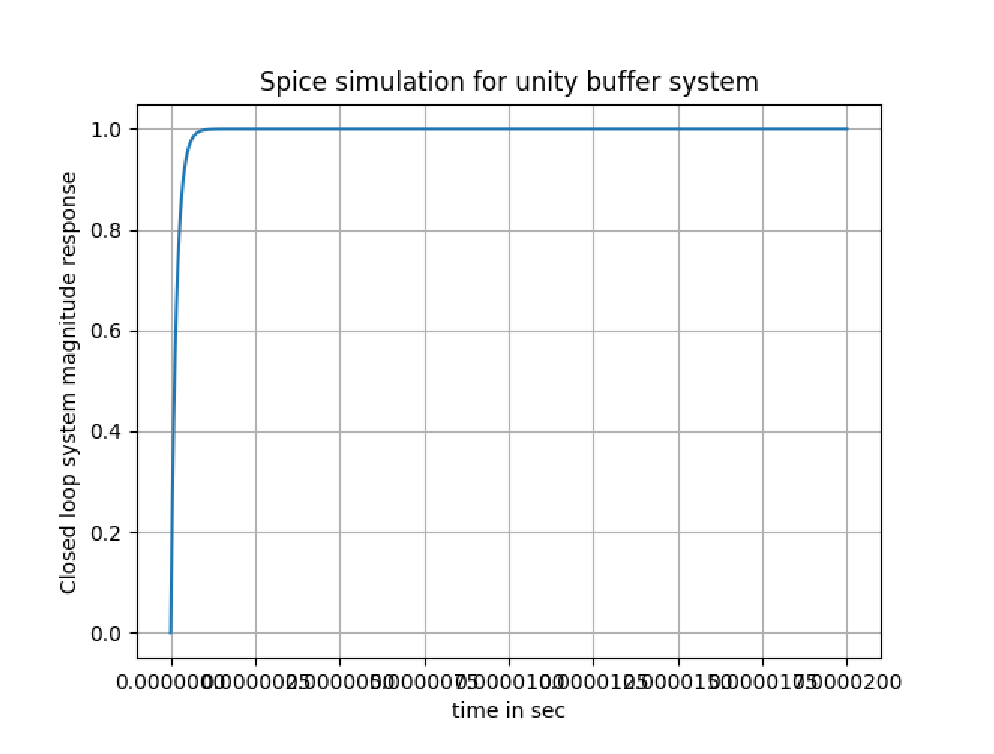
\includegraphics[width=\columnwidth]{./figs/ee18btech11012_1/ee18btech11012_spiceresult.eps}
\caption{}
\label{fig:ee18btech11012_spiceresult}
\end{figure}
\item The following python code plots the closed loop response verses time and the python plot is also shown below.
\begin{lstlisting}
spice/ee18btech11012/ee18btech11012_spiceresult1.py
\end{lstlisting}
\begin{figure}[!h]
\centering
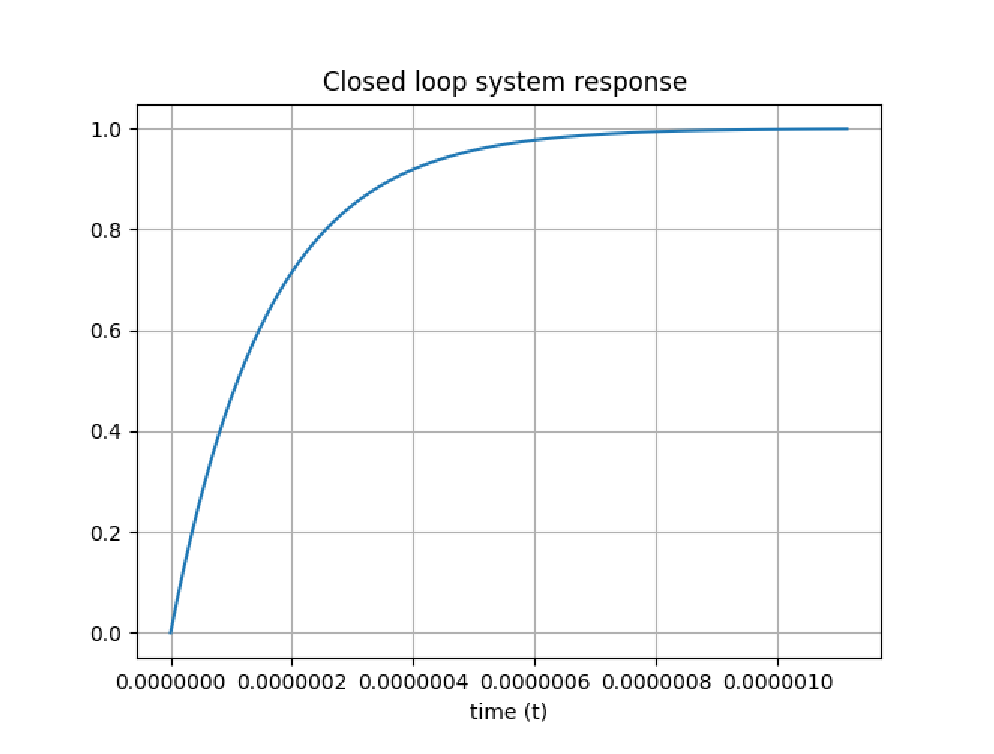
\includegraphics[width=\columnwidth]{./figs/ee18btech11012_1/ee18btech11012_spiceresult1.eps}
\caption{}
\label{fig:ee18btech11012_spiceresult1}
\end{figure}

\end{enumerate}
